%% March 2018
%%%%%%%%%%%%%%%%%%%%%%%%%%%%%%%%%%%%%%%%%%%%%%%%%%%%%%%%%%%%%%%%%%%%%%%%%%%%
% AGUJournalTemplate.tex: this template file is for articles formatted with LaTeX
%
% This file includes commands and instructions
% given in the order necessary to produce a final output that will
% satisfy AGU requirements, including customized APA reference formatting.
%
% You may copy this file and give it your
% article name, and enter your text.
%
%
% Step 1: Set the \documentclass
%
% There are two options for article format:
%
% PLEASE USE THE DRAFT OPTION TO SUBMIT YOUR PAPERS.
% The draft option produces double spaced output.
%

%% To submit your paper:
\documentclass[draft,linenumbers]{agujournal2018}
\usepackage{apacite}
\usepackage{url} %this package should fix any errors with URLs in refs.
%%%%%%%
% As of 2018 we recommend use of the TrackChanges package to mark revisions.
% The trackchanges package adds five new LaTeX commands:
%
%  \note[editor]{The note}
%  \annote[editor]{Text to annotate}{The note}
%  \add[editor]{Text to add}
%  \remove[editor]{Text to remove}
%  \change[editor]{Text to remove}{Text to add}
%
% complete documentation is here: http://trackchanges.sourceforge.net/
%%%%%%%


%% Enter journal name below.
%% Choose from this list of Journals:
%
% JGR: Atmospheres
% JGR: Biogeosciences
% JGR: Earth Surface
% JGR: Oceans
% JGR: Planets
% JGR: Solid Earth
% JGR: Space Physics
% Global Biogeochemical Cycles
% Geophysical Research Letters
% Paleoceanography and Paleoclimatology
% Radio Science
% Reviews of Geophysics
% Tectonics
% Space Weather
% Water Resources Research
% Geochemistry, Geophysics, Geosystems
% Journal of Advances in Modeling Earth Systems (JAMES)
% Earth's Future
% Earth and Space Science
% Geohealth
%
% ie, \journalname{Water Resources Research}

\journalname{Geophysical Research Letters}


\usepackage{soulutf8}

\begin{document}

%% ------------------------------------------------------------------------ %%
%  Title
%
% (A title should be specific, informative, and brief. Use
% abbreviations only if they are defined in the abstract. Titles that
% start with general keywords then specific terms are optimized in
% searches)
%
%% ------------------------------------------------------------------------ %%

% Example: \title{This is a test title}

\title{Spatiotemporal Assessments of Greenhouse Gas Concentration and Flux in
Headwater Tropical Streams}

%% ------------------------------------------------------------------------ %%
%
%  AUTHORS AND AFFILIATIONS
%
%% ------------------------------------------------------------------------ %%

% Authors are individuals who have significantly contributed to the
% research and preparation of the article. Group authors are allowed, if
% each author in the group is separately identified in an appendix.)

% List authors by first name or initial followed by last name and
% separated by commas. Use \affil{} to number affiliations, and
% \thanks{} for author notes.
% Additional author notes should be indicated with \thanks{} (for
% example, for current addresses).

% Example: \authors{A. B. Author\affil{1}\thanks{Current address, Antartica}, B. C. Author\affil{2,3}, and D. E.
% Author\affil{3,4}\thanks{Also funded by Monsanto.}}

\authors{
Andrew R. Murray
\affil{1}
Keridwen Whitmore
\affil{1}
Diego Riveros-Iregui
\affil{1}
Andrea Encalada
\affil{2}
Esteban Suarez
\affil{2}
Gonzalo Rivas-Torres
\affil{2}
}


% \affiliation{1}{First Affiliation}
% \affiliation{2}{Second Affiliation}
% \affiliation{3}{Third Affiliation}
% \affiliation{4}{Fourth Affiliation}

\affiliation{1}{University of North Carolina - Chapel Hill Department of Geography}
\affiliation{2}{Universidad de San Francisco de Quito}
%(repeat as many times as is necessary)

%% Corresponding Author:
% Corresponding author mailing address and e-mail address:

% (include name and email addresses of the corresponding author.  More
% than one corresponding author is allowed in this LaTeX file and for
% publication; but only one corresponding author is allowed in our
% editorial system.)

% Example: \correspondingauthor{First and Last Name}{email@address.edu}
\correspondingauthor{Andrew Murray}{armurray@live.unc.edu}

%% Keypoints, final entry on title page.

%  List up to three key points (at least one is required)
%  Key Points summarize the main points and conclusions of the article
%  Each must be 100 characters or less with no special characters or punctuation

% Example:
% \begin{keypoints}
% \item	List up to three key points (at least one is required)
% \item	Key Points summarize the main points and conclusions of the article
% \item	Each must be 100 characters or less with no special characters or punctuation
% \end{keypoints}

\begin{keypoints}
\item Streams in the Páramo region are carbon sources.
\item Variability in carbon evasion is driven by discharge and slope.
\item CO\textsubscript{2} evasion can be quantified with a minimal appraoch.
\end{keypoints}

%% ------------------------------------------------------------------------ %%
%
%  ABSTRACT
%
% A good abstract will begin with a short description of the problem
% being addressed, briefly describe the new data or analyses, then
% briefly states the main conclusion(s) and how they are supported and
% uncertainties.
%% ------------------------------------------------------------------------ %%

%% \begin{abstract} starts the second page

\begin{abstract}
Long thought to be a carbon sink, the Páramo region of the Andes may be
a significant carbon source. We evaluated the spatiotemporal dynamics of
CO\textsubscript{2} concentration and flux in a high-elevation stream.
We measured 15-min dissolved CO\textsubscript{2}, O\textsubscript{2},
and discharge, across a wetland-stream transition, characteristic of
tropical, alpine environments.
\end{abstract}
\noindent{\bf Plain language summary}\vskip-\parskip

\noindent{Streams emit carbon dioxide to the atmosphere, but how much? Recent
research suggests that steaper streams emit more carbon dioxide since
they are more turbulent, but the amount of carbon dioxide a stream emits
is also dependent on the carbon content of the local ecosystem. The
paramo, which is a region in the high Andes mountains in Peru, Ecuador
and Columbia, above the treeline (\textasciitilde{} 10,000 ft) and below
the snow line (\textasciitilde{} 16,000 ft), is made up of extensive
peatlands which hold enormous amounts of carbon. In the past, it was
believed that the paramo took in carbon from the atmosphere and stored
it however, recent research suggests that the region has reversed course
and is now emitting more carbon into the atmosphere than it is taking
in. A principal way that carbon is moved from the soils into the
atmosphere is through the water cycle. We set up a sensor network in a
stream in the Ecuadorian paramo to measure changes in carbon dioxide and
dissolved oxygen, while also recording stream discharge. We then took
this data and created a method for determining how much carbon dioxide
is being emitted from the stream to the atmosphere and how that relates
to discharge, steepness of the stream, and precipitation.}
\vskip18pt
\section{Introduction}

It is well known that CO\textsubscript{2} flux from freshwater streams
impacts the global carbon cycle, however our ability to quantify these
affects at a variety of spatial and temporal scales remains limited. The
Páramo has historically been thought to be a carbon sink however, recent
research suggests that it is now a source of carbon to the atmosphere
\citep{carrillO2019breathing}. We tested two methods of quantifying
CO\textsubscript{2} evasion in headwater streams in the Páramo region of
Ecuador and discuss the results and implications of our findings. We
utilized eosense EosFD flux chamber sensors to measure
CO\textsubscript{2} flux directly from streams using in-stream flotation
devices. Additionally, we used multiple Vaisala CO\textsubscript{2}
concentration sensors, fitted with waterproof PTFE sleeves to monitor
change in in-stream concentration and calculated flux by converting
concentration to mass per area time using the formula:

\begin{linenomath*}
\begin{equation}
f=\frac{\Delta ppm}{A}*.0018*\frac{10^6}{44.01}*Q+(R-P)
\end{equation}
\end{linenomath*}

Where \(f\) equals flux in \(µmol\:m^{-2}s^{-1}\), \(\Delta ppm\) is the
change in CO\textsubscript{2} ppm between sensors, \(R\) is stream
respiration in ppm, \(P\) is gross primary production in ppm, A is the
stream surface area between sensors in \(m^2\), .0018 is the conversion
coefficient for \(CO_2\) from ppm to \(g\:m^{-3}\) and 44.01 is the
molar mass of \(CO_2\).

\subsection{Background}

The Páramo region is characterized by high elevation, mountainous
wetlands that are connected by turbulent streams. Connectivity can be
seasonal and dependent upon precipitation intensity. Our specific site
lies on the western edge of the Andean continental divide. The site
receives mean monthly precipitation of 121 mm (Standard deviation =
61mm). Precipitation is moderately seasonal with maximum precipitation
typically occurring in July and minimum precipitation in February. The
site experiences some level of precipitation on 83.5\% of days. Mean
daily temperature is 50 C. We instrumented a reach approximately 140
meters in length which serves as a direct outlet to a wetland with an
area of 2.3 Ha as well as multiple additional wetlands further upstream.
Four sensor clusters were installed at various intervals representing
various stream gradients (figure 1). A waterfall measuring
\textasciitilde{}4m exists between station 3 and 4.

\section{Methods}

Four Vaisala GM-220 CO\textsubscript{2} sensors were used to measure
dissolved in-stream CO\textsubscript{2} concentrations. We used
waterproof PTFE sleeves, following the method presented in Johnson., et
al.(2010). The Vaisala sensors, which have a range of 0-10,000 ppm, have
a margin of error of 150 ppm (1.5\%). To minimize error, all four
sensors were initially collocated to establish offset values. Two eosFD
(EoSense) chamber sensors were positioned in the stream using custom
made floating platforms. One sensor was located between Station 1 and 2,
and the other was collocated with station 4. To estimate evasion from
the reach, we quantified CO\textsubscript{2} change between station 1
and 4.

\begin{figure}[h]
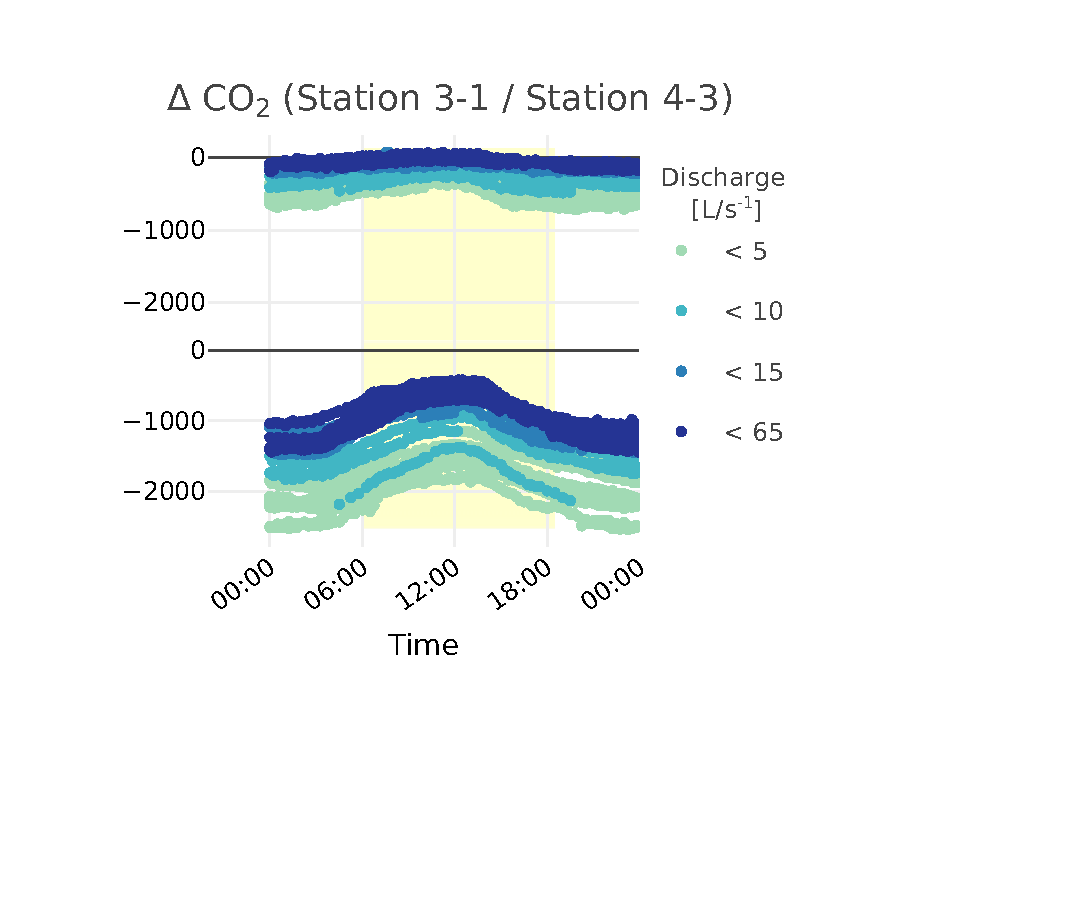
\includegraphics{StreamFluxArticle_files/figure-latex/filt14PpmPlot-1} \caption{This is that real nice caption!}\label{fig:filt14PpmPlot}
\end{figure}

\section{Data}

\section{Results}

\section{Conclusions}

\acknowledgments

Data, as well as all scripts for conducting this analysis are hosted on
GitHub and can be obtained at:
https://github.com/ARMurray/Ecuador/tree/master/Articles/StreamFluxArticle

This work was funded by the National Science Foundation under award
1847331: \emph{The role of small wetland connectivity in controlling
greenhouse gas emissions and downstream carbon fluxes from headwater
tropical streams.}

The authors would like to thank:

La Universidad de San Francisco de Quito for their material and
institutional support throughout this research.

\section{Reminders}

\subsection{How to cite}

Please use ONLY \textbackslash{}citet and \textbackslash{}citep for
reference citations. DO NOT use other cite commands (e.g.,
\textbackslash{}cite, \textbackslash{}citeyear, \textbackslash{}nocite,
\textbackslash{}citealp, etc.). Example \textbackslash{}citet and
\textbackslash{}citep: \ldots{}as shown by \citet{Levitus2012},
\citet{NunciO2011} and \citet{Raphael2004} \ldots{}as shown by
\citep{Levitus2012}, \citep{NunciO2011}, \citep{Raphael2004}.
\ldots{}has been shown
\citep[e.g.,][]{Levitus2012, NunciO2011, Raphael2004}.

\bibliography{references.bib}


\end{document}
